\everymath{\displaystyle}
\documentclass{beamer}
% \documentclass[handout]{beamer}

%\usepackage[pdftex]{color,graphicx}
\usepackage{amsmath,amssymb,amsfonts}

\mode<presentation>
{
  % \usetheme{Darmstadt}
  % \usetheme[hideothersubsections]{Hannover}
  % \usetheme[hideothersubsections]{Goettingen}
  \usetheme[hideothersubsections, right]{Berkeley}

  \usecolortheme{seahorse}
  % \usecolortheme{dolphin}
  \usecolortheme{rose}
  % \usecolortheme{orchid}

  \useinnertheme[shadow]{rounded}

  \setbeamercovered{transparent}
  % or whatever (possibly just delete it)
}

\mode<handout>{
  \setbeamercolor{background canvas}{bg=black!5}
  \usepackage{pgfpages}
  \pgfpagesuselayout{4 on 1}[a4paper,border shrink=5mm, landscape]
}

\usepackage[brazilian]{babel}
% or whatever

% \usepackage[latin1]{inputenc}
\usepackage[utf8]{inputenc}
% or whatever

\usepackage{times}
%\usepackage[T1]{fontenc}
% Or whatever. Note that the encoding and the font should match. If T1
% does not look nice, try deleting the line with the fontenc.


\title%[] % (optional, use only with long paper titles)
{A distribuição Normal}

\subtitle
{Distribuição Normal, e IC da média} % (optional)

\author%[] % (optional, use only with lots of authors)
{Felipe Figueiredo}% \and S.~Another\inst{2}}
% - Use the \inst{?} command only if the authors have different
%   affiliation.

\institute[] % (optional, but mostly needed)
{
}
  % \inst{1}%
  % Department of Computer Science\\
  % University of Somewhere
  % \and
  % \inst{2}%
  % Department of Theoretical Philosophy\\
  % University of Elsewhere}
% - Use the \inst command only if there are several affiliations.
% - Keep it simple, no one is interested in your street address.

\date%[] % (optional)
{}

% \subject{Talks}
% This is only inserted into the PDF information catalog. Can be left
% out. 



% If you have a file called "university-logo-filename.xxx", where xxx
% is a graphic format that can be processed by latex or pdflatex,
% resp., then you can add a logo as follows:

\pgfdeclareimage[height=1.6cm]{university-logo}{../logo}
\logo{\pgfuseimage{university-logo}}



% Delete this, if you do not want the table of contents to pop up at
% the beginning of each subsection:
\AtBeginSubsection[]
%\AtBeginSection[]
{
  \begin{frame}<beamer>{Sumário}
    \tableofcontents[currentsection,currentsubsection]
  \end{frame}
}


% If you wish to uncover everything in a step-wise fashion, uncomment
% the following command: 

% \beamerdefaultoverlayspecification{<+->}


\begin{document}

\begin{frame}
  \titlepage
\end{frame}

\begin{frame}{Sumário}
  \tableofcontents
  % You might wish to add the option [pausesections]
\end{frame}


%% Template
% \section{}

% \subsection{}

% \begin{frame}{}
%   \begin{itemize}
%   \item 
%   \end{itemize}
% \end{frame}

% \begin{frame}
%   \begin{columns}
%     \begin{column}{5cm}
%     \end{column}
%     \begin{column}{5cm}
%     \end{column}
%   \end{columns}
% \end{frame}

% \begin{frame}{}
%   \includegraphics[height=0.4\textheight]{file1}
%   \includegraphics[height=0.4\textheight]{file2}
%   \includegraphics[height=0.4\textheight]{file3}
%   \begin{figure}
%     \caption{}
%   \end{figure}
% \end{frame}

% \begin{frame}{}
%   \begin{definition}
%   \end{definition}
%   \begin{example}
%   \end{example}
%   \begin{block}{Exercício}
%   \end{block}
% \end{frame}

\section{Discussão da aula passada}

\subsection{Discussão da aula passada}

\begin{frame}{Discussão da aula passada}
  \begin{block}{}
    Discussão da leitura obrigatória da aula passada
  \end{block}
\end{frame}

\section{A distribuição Normal}

\subsection{Distribuições de probabilidade}

\begin{frame}{Recapitulando}
  \begin{columns}
    \begin{column}{5cm}
      \begin{itemize}
      \item (aula passada)
      \item Pressão sanguínea (PS) de todos os 100 alunos de uma sala
      \item Visualização da média e variabilidade dos dados
      \end{itemize}
    \end{column}
    \begin{column}{5cm}
      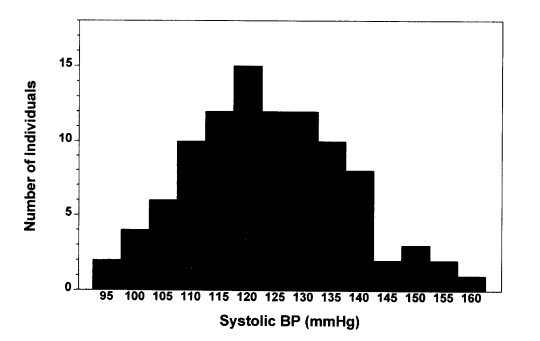
\includegraphics[width=\textwidth]{Cap3/histograma1}
    \end{column}
  \end{columns}
\end{frame}

\begin{frame}{Distribuições de probabilidade - Por que?}
  \begin{itemize}
  \item Distribuições teóricas = \alert{modelos} da realidade
  \item Aprender com os modelos $\Rightarrow$ ferramenta
  \end{itemize}
  \begin{block}{Na vida real}
    Distribuição ``próxima'' de um modelo $\Rightarrow$ metodologia
  \end{block}
\end{frame}

\begin{frame}[label=exemplo5.1]{Distribuições de dados ``reais''}
  \begin{exampleblock}{Exemplo 5.1}
    No exemplo, a PS dos 100 alunos (a turma inteira) foi visualizada em um histograma.

    Calculando a média, encontramos $\bar{x}$ = 123,4 mmHg.

    Calculando o DP, encontramos $s$ = 14,0 mmHg.
  \end{exampleblock}
  \begin{block}{Pense...}
    \begin{itemize}
    \item Se a população for a turma, sabemos a média e o DP {\bf com certeza}
    \item Se a turma é uma amostra de uma população maior, como podemos {\em inferir} os parâmetros da população (digamos, com 95\% de confiança)?
    \end{itemize}
  \end{block}
\end{frame}

\begin{frame}{Distribuições de dados ``reais''}
  \begin{columns}
    \begin{column}{5cm}
      \begin{exampleblock}{Exemplo 5.1}
        \begin{itemize}
        \item $\bar{x}$ = 123,4 mmHg
        \item $s$ = 14,0 mmHg
        \end{itemize}
      \end{exampleblock}
      \begin{block}{}
        \begin{itemize}
        \item Você  {\em vê} a média?
        \item Você  {\em vê} o DP?
        \end{itemize}
      \end{block}
    \end{column}
    \begin{column}{5cm}
      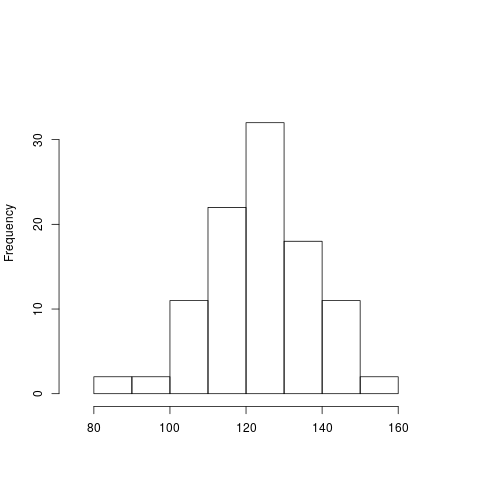
\includegraphics[width=\textwidth]{Cap4/normal1}
    \end{column}
  \end{columns}
\end{frame}

\begin{frame}{Observações importantes}
  \begin{columns}
    \begin{column}{5cm}
      \begin{itemize}
      \item Muitas medições próximas da média
      \item Poucas medições de PS muito baixas
      \item Poucas medições de PS muito altas
      \item Aprox. simétrica em torno da média
      \end{itemize}
    \end{column}
    \begin{column}{5cm}
      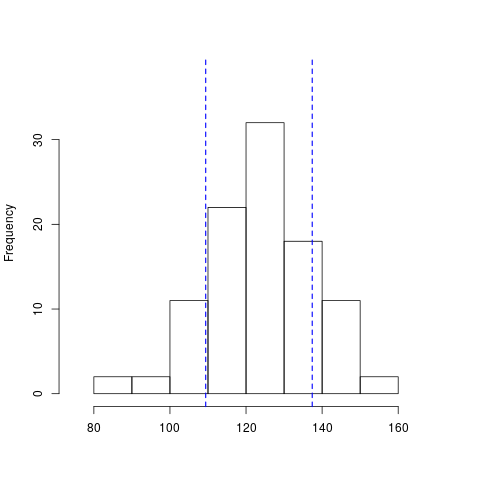
\includegraphics[width=\textwidth]{Cap4/normal3}
    \end{column}
  \end{columns}
\end{frame}

\subsection{A distribuição Normal}


\begin{frame}{Distribuição Normal}
  \begin{center}
    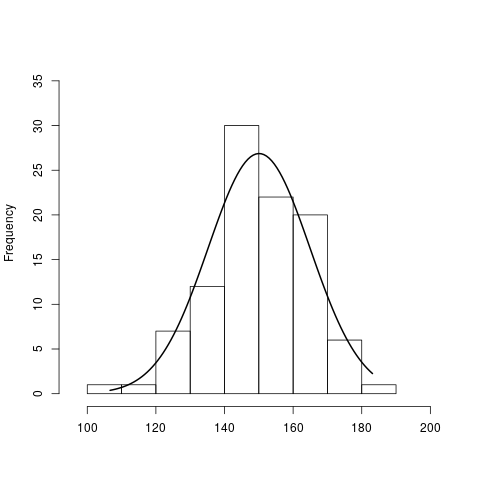
\includegraphics[height=\textheight]{Cap4/normal2}
  \end{center}
\end{frame}

\begin{frame}{Distribuição Normal, com DP}
  \begin{center}
    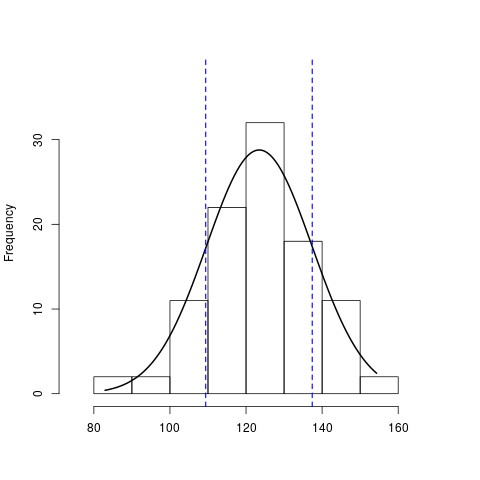
\includegraphics[height=\textheight]{Cap4/normal4}
  \end{center}
\end{frame}

\begin{frame}{E esta?}
  \begin{columns}
    \begin{column}{5cm}
      \begin{itemize}
      \item Muitas medições próximas da média?
      \item Poucas medições de PS muito baixas?
      \item Poucas medições de PS muito altas?
      \item Aprox. simétrica em torno da média?
      \end{itemize}
    \end{column}
    \begin{column}{5cm}
      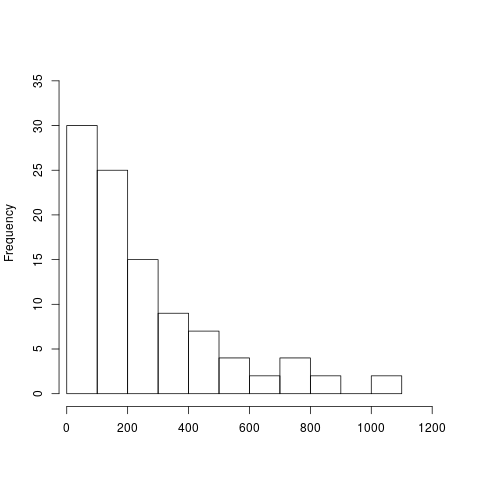
\includegraphics[width=\textwidth]{Cap4/lognormal}
    \end{column}
  \end{columns}
\end{frame}

\begin{frame}{E esta?}
  \begin{columns}
    \begin{column}{5cm}
      \begin{itemize}
      \item Muitas medições próximas da média?
      \item Poucas medições de PS muito baixas?
      \item Poucas medições de PS muito altas?
      \item Aprox. simétrica em torno da média?
      \end{itemize}
    \end{column}
    \begin{column}{5cm}
      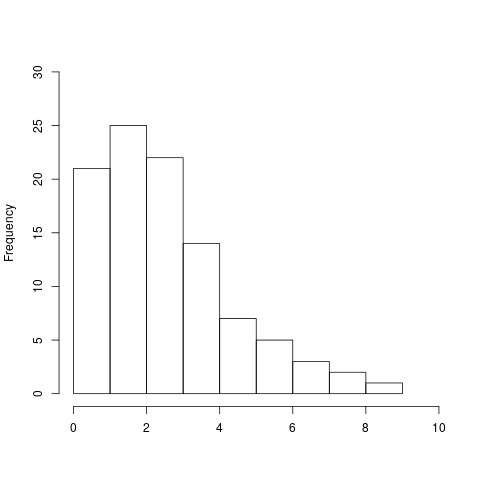
\includegraphics[width=\textwidth]{Cap4/poisson}
    \end{column}
  \end{columns}
\end{frame}

\begin{frame}{E esta?}
  \begin{columns}
    \begin{column}{5cm}
      \begin{itemize}
      \item Muitas medições próximas da média?
      \item Poucas medições de PS muito baixas?
      \item Poucas medições de PS muito altas?
      \item Aprox. simétrica em torno da média?
      \end{itemize}
    \end{column}
    \begin{column}{5cm}
      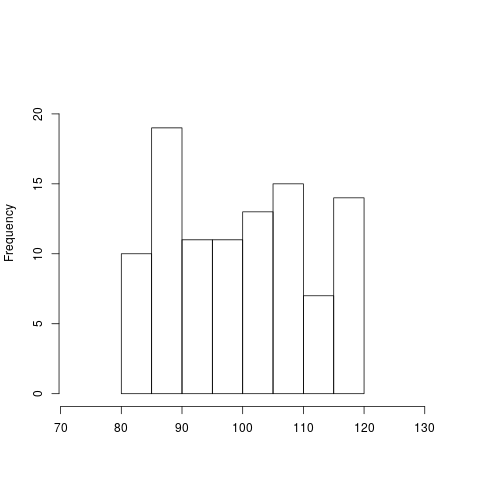
\includegraphics[width=\textwidth]{Cap4/uniforme}
    \end{column}
  \end{columns}
\end{frame}

\subsection{Inferências}

\begin{frame}{A regra empírica}
  \begin{itemize}
  \item (aula passada)
  \item ``mais da metade'' dos dados estão a 1 DP da média
  \item ``quase todos'' os dados estão a 2 DPs da média
  \end{itemize}
\end{frame}

\begin{frame}{A regra empírica}
  \begin{columns}
    \begin{column}{5cm}
      \begin{itemize}
      \item 68\% a até 1 DP da média
      \item 95\% a até 2 DP da média
      \item 99,7\% a até 3 DP da média
      \end{itemize}
    \end{column}
    \begin{column}{5cm}
      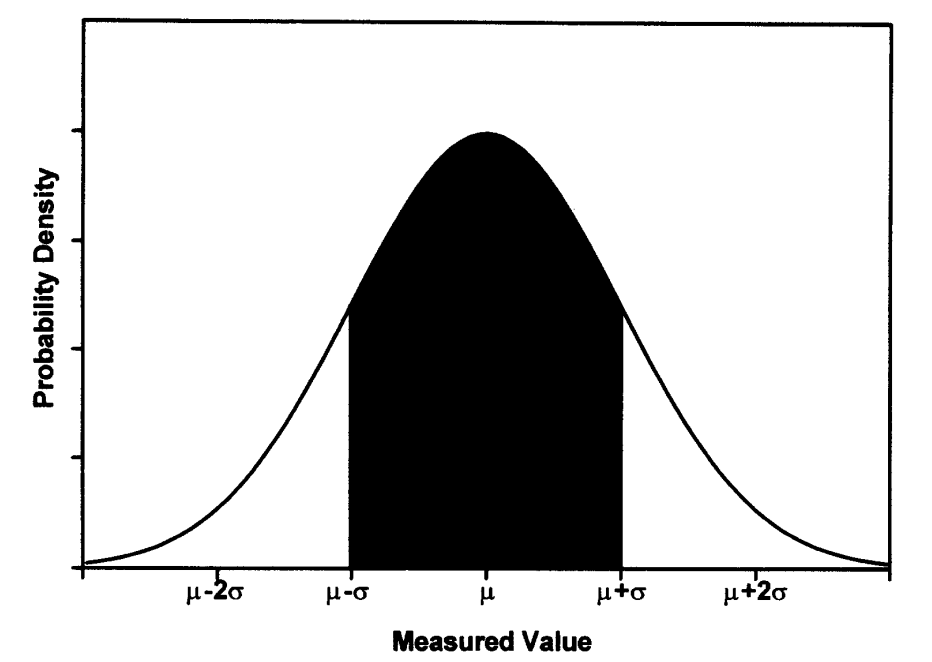
\includegraphics[width=\textwidth]{Cap4/empirica}
    \end{column}
  \end{columns}
\end{frame}

\section{IC da média}

\subsection{Interpretação}

\begin{frame}{Exemplos}
  \begin{center}
    Vamos recapitular o exemplo 5.1, antes de introduzir outro.
  \end{center}
\end{frame}

\againframe{exemplo5.1}

\begin{frame}{Distribuições de dados ``reais''}
  \begin{exampleblock}{Exemplo 5.2}
    Das 100 medições de PS, você amostrou aleatoriamente 5 medições.

    Valores aproximados: 120, 80, 90, 110 e 95 mmHg.

    Calculando a média, encontramos $\bar{x}$ = 99,0 mmHg.

    Calculando o DP, encontramos $s$ = 15,97 mmHg.
  \end{exampleblock}
  \begin{block}{Pense...}
    \begin{itemize}
    \item Se a população for a turma, podemos estimar a média e o DP da turma com os valores desta amostra?
    \item Se a turma é uma amostra de uma população maior, esta estimativa nos dá ``mais confiança'' sobre a população, ou menos?
    \end{itemize}
  \end{block}
\end{frame}

\begin{frame}{IC da média}
  \begin{exampleblock}{ICs dos exemplos}
    \begin{itemize}
    \item O IC do exemplo 5.1: 120,6 até 126,2 mmHg
    \item O IC do exemplo 5.2: 79,2 até 118,8 mmHg
    \end{itemize}
  \end{exampleblock}
  \begin{block}{Relembre...}<2->
    O que significa o IC?
  \end{block}
  \begin{block}{Pense...}
    Observe os tamanhos dos ICs.
  \end{block}
\end{frame}

\subsection{Premissas}

\begin{frame}{Premissas}
  Assumimos que estas coisas são verdadeiras para calcular/interpretar um IC
  \begin{itemize}
  \item A amostra foi selecionada aleatoriamente da população (sem reposição)
  \item A população é Normal (Gaussiana)
  \item Os indivíduos são independentes, uns dos outros
  \end{itemize}
\end{frame}

\subsection{O Erro Padrão}

\begin{frame}{Teorema do Limite Central}
  Vídeo
\end{frame}

\begin{frame}{ Variabilidade x Erro Padrão}
  \begin{block}{Variabilidade}
    A variabilidade nos informa sobre a dispersão da amostra/população.
  \end{block}
  \begin{block}{O erro padrão}
    O Erro Padrão nos informa quão boa é nossa \alert{estimativa} da média.
  \end{block}
\end{frame}

\begin{frame}{O Erro Padrão - definição}
  \begin{displaymath}
    SEM = \frac{s}{\sqrt{n}}
  \end{displaymath}
  \begin{itemize}
  \item SEM = Erro Padrão da Média (em inglês)
  \item Conforme $n$ aumenta $\Rightarrow$ SEM diminui
  \item Conforme $n$ aumenta $\Rightarrow$ $\bar{x}$ ``próximo'' de $\mu$
  \end{itemize}
  \begin{block}{Lembrete}
    \begin{itemize}
    \item $\bar{x}$ -- média da amostra (resultado/possível)
    \item $\mu$ -- média da população (objetivo/inferência)
    \end{itemize}
  \end{block}
\end{frame}

\begin{frame}{O Erro Padrão - Interpretação}
  \begin{block}{Interpretação}
    Quando queremos {\bf inferir} a média da população a partir de uma amostra, qual é a incerteza associada a esta estimativa?
  \end{block}
  \begin{block}{Pense...}<2->
    E o desvio-padrão $s$?
  \end{block}
\end{frame}

\begin{frame}{O Erro Padrão}
  \begin{displaymath}
    IC: \bar{x} \pm t^{*} \times SEM
  \end{displaymath}
  \begin{itemize}
  \item $\bar{x}$ = média
  \item Para amostras {\bf grandes}, $t^{*} \approx$ 2.
  \end{itemize}
\end{frame}

\begin{frame}{O Erro Padrão - IC da média}
  \begin{displaymath}
    IC: \bar{x} \pm t^{*} \times SEM
  \end{displaymath}
  \begin{block}{Perguntas}
    \begin{enumerate}
    \item<1-> Se $s$ aumenta, o SEM aumenta ou diminui?
    \item<2-> Se $s$ aumenta, o IC aumenta ou diminui?
    \item<3-> Se $t^{*}$ aumenta, o IC aumenta ou diminui?
    \end{enumerate}
  \end{block}
\end{frame}

\begin{frame}{O Erro Padrão}
  \begin{displaymath}
    IC: \bar{x} \pm 2\footnote{$t^{*} \approx$ 2} \times SEM
  \end{displaymath}
  \begin{exampleblock}{Exemplo 5.1}
    \begin{itemize}
    \item $s$ = 14,0 e N = 100
    \item $SEM = \frac{14}{\sqrt{100}} = 1.4$
    \item IC =  $123.4 \pm 2 \times 1.4$
    \item IC =  $123.4 \pm 2.8$
    \bigskip
    \item IC $\approx$ [120.6, 126.2]
    \end{itemize}
  \end{exampleblock}
\end{frame}

\begin{frame}{Pense...}
  \begin{exampleblock}{}
    \begin{itemize}
    \item {\bf Ex. 5.1:} $\bar{x}$ = 123,4 e $s$ = 14,0 mmHg ($N=100$)
    \item {\bf Ex. 5.2:} $\bar{x}$ = 99,0 e $s$ = 15,97 mmHg ($N=5$)
    \end{itemize}
  \end{exampleblock}
  \begin{block}{Podemos reproduzir o mesmo método do 5.1 no 5.2?}
  \begin{itemize}
  \item SEM do exemplo 5.1 = 1,4
  \item SEM do exemplo 5.2 = 6,3?
  \end{itemize}
  \end{block}
\end{frame}

\begin{frame}{}
    \begin{block}{Podemos reproduzir o mesmo método do 5.1 no 5.2?}
  \begin{itemize}
  \item SEM do exemplo 5.1 = 1,4
  \item SEM do exemplo 5.2 = 6,3?
  \end{itemize}
  \end{block}
  \begin{block}{Resposta}
    Não! Pois N=5 não é grande!

    \bigskip
    Isso faz com que o SEM do exemplo 5.2 seja muito maior (como vimos).
  \end{block}
  \begin{exampleblock}{Lembrete -- ICs dos exemplos}
    \begin{itemize}
    \item O IC do exemplo 5.1: 120,6 -- 126,2 mmHg
    \item O IC do exemplo 5.2: 79,2 -- 118,8 mmHg
    \end{itemize}
  \end{exampleblock}
\end{frame}

\begin{frame}
  \begin{exampleblock}{Lembrete -- ICs dos exemplos}
    \begin{itemize}
    \item O IC do exemplo 5.1: 120,6 -- 126,2 mmHg
    \item O IC do exemplo 5.2: \alert{79,2 -- 118,8 mmHg}
    \end{itemize}
  \end{exampleblock}
  \begin{block}{No caso do exemplo 5.2}
    \begin{itemize}
    \item $\bar{x} = 99$ mmHg
    \item O SEM proposto no slide anterior é $\approx$ 6 mmHg
    \item A margem de erro seria {\bf 2} $\times $ 6 $\approx$ 12 mmHg
    \end{itemize}
      $\Rightarrow$ O IC proposto seria \alert{87 -- 111 mmHg}
  \end{block}
  \begin{block}{Pense...}
    Qual parece ser a margem de erro {\em real} do IC acima?
  \end{block}
\end{frame}

\begin{frame}
  \begin{exampleblock}{Lembrete -- ICs dos exemplos}
    \begin{itemize}
    \item O IC do exemplo 5.1: 120,6 -- 126,2 mmHg
    \item O IC do exemplo 5.2: \alert{79,2 -- 118,8 mmHg}
    \end{itemize}
  \end{exampleblock}
  \begin{block}{No caso do exemplo 5.2}
    \begin{itemize}
    \item O IC proposto seria \alert{87 -- 111 mmHg}
    \end{itemize}
  \end{block}
  \begin{block}{Pense...}
    Qual é a sua conclusão sobre esse $t^{*}$ misterioso?
  \end{block}
\end{frame}

\section{Aprofundamento}

\subsection{Aprofundamento}

\begin{frame}{Aprofundamento}
  \begin{block}{Leitura obrigatória}
    Capítulo 4. Pular a seção {\bf Intervalo de Predição}.

    Capítulo 5. Pular as seções:
    \begin{itemize}
    \item Calculando o IC da média
    \item A distribuição {\em t} (será abordado na próxima aula)
    \end{itemize}

  \end{block}
  \begin{block}{Leitura recomendada}
    Capítulo 4. seção {\bf Intervalo de Predição}.
  \end{block}
  \begin{itemize}
  \item Cap 4: Exercícios 1, 2 e 3.
  \item Cap 5: exercícios 1, 3, 7 e 9.
  % \item Cap 5: exercício 5, item A. Use $t^{*}$ = 2.
  \end{itemize}
\end{frame}

\end{document}
